\begin{figure}[H]
    \centering
    \begin{adjustbox}{max width=\textwidth}
    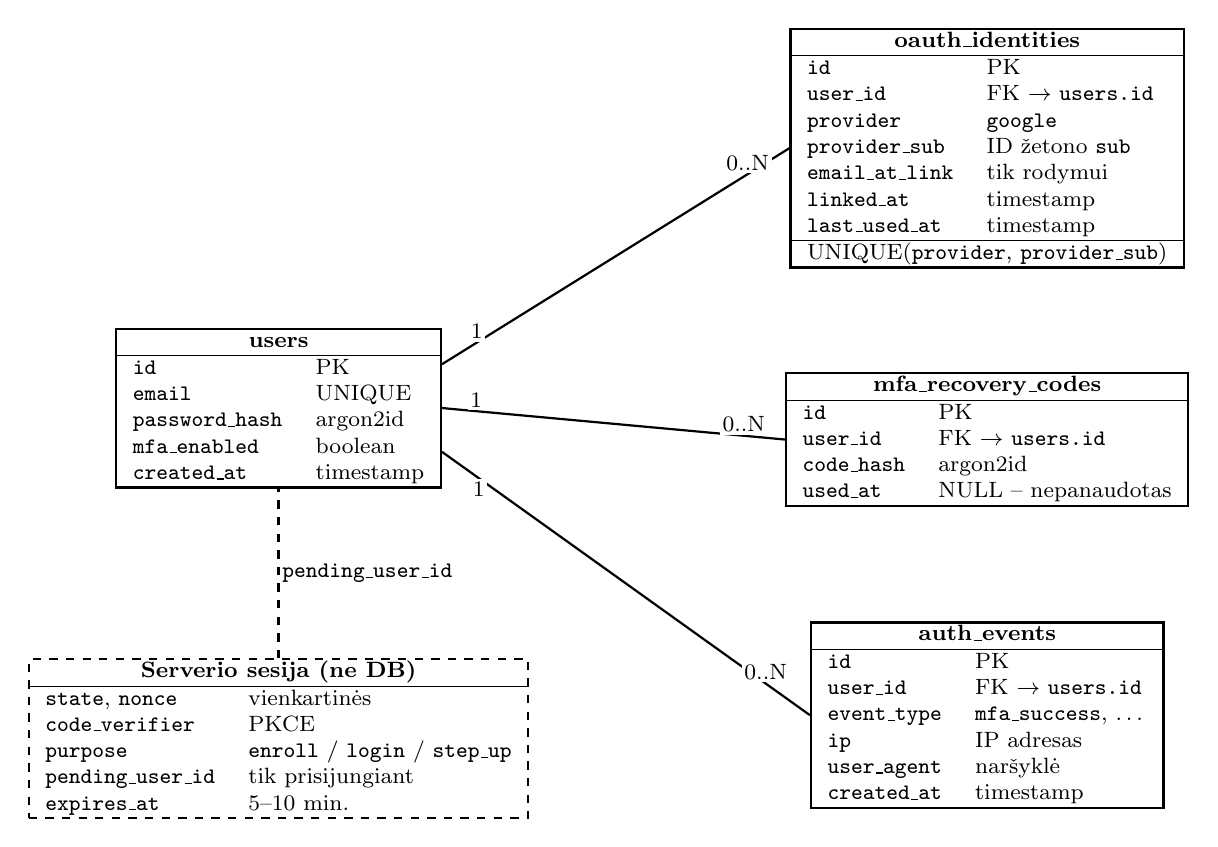
\begin{tikzpicture}[
        entity/.style={draw, thick, fill=white, inner sep=0pt, font=\footnotesize},
        session/.style={draw, thick, dashed, fill=white, inner sep=0pt, font=\footnotesize},
        rel/.style={thick},
        card/.style={font=\footnotesize, fill=white, inner sep=1pt},
    ]
        \node[entity] (users) at (0,0) {%
            \begin{tabular}{l l}
                \multicolumn{2}{c}{\textbf{users}} \\ \hline
                \texttt{id}             & PK \\
                \texttt{email}          & UNIQUE \\
                \texttt{password\_hash} & argon2id \\
                \texttt{mfa\_enabled}   & boolean \\
                \texttt{created\_at}    & timestamp \\
            \end{tabular}};

        \node[entity] (oauth) at (9,3.3) {%
            \begin{tabular}{l l}
                \multicolumn{2}{c}{\textbf{oauth\_identities}} \\ \hline
                \texttt{id}              & PK \\
                \texttt{user\_id}        & FK $\to$ \texttt{users.id} \\
                \texttt{provider}        & \texttt{google} \\
                \texttt{provider\_sub}   & ID žetono \texttt{sub} \\
                \texttt{email\_at\_link} & tik rodymui \\
                \texttt{linked\_at}      & timestamp \\
                \texttt{last\_used\_at}  & timestamp \\ \hline
                \multicolumn{2}{l}{UNIQUE(\texttt{provider}, \texttt{provider\_sub})} \\
            \end{tabular}};

        \node[entity] (codes) at (9,-0.4) {%
            \begin{tabular}{l l}
                \multicolumn{2}{c}{\textbf{mfa\_recovery\_codes}} \\ \hline
                \texttt{id}         & PK \\
                \texttt{user\_id}   & FK $\to$ \texttt{users.id} \\
                \texttt{code\_hash} & argon2id \\
                \texttt{used\_at}   & NULL -- nepanaudotas \\
            \end{tabular}};

        \node[entity] (events) at (9,-3.9) {%
            \begin{tabular}{l l}
                \multicolumn{2}{c}{\textbf{auth\_events}} \\ \hline
                \texttt{id}          & PK \\
                \texttt{user\_id}    & FK $\to$ \texttt{users.id} \\
                \texttt{event\_type} & \texttt{mfa\_success}, \ldots \\
                \texttt{ip}          & IP adresas \\
                \texttt{user\_agent} & naršyklė \\
                \texttt{created\_at} & timestamp \\
            \end{tabular}};

        \node[session] (sess) at (0,-4.2) {%
            \begin{tabular}{l l}
                \multicolumn{2}{c}{\textbf{Serverio sesija (ne DB)}} \\ \hline
                \texttt{state}, \texttt{nonce} & vienkartinės \\
                \texttt{code\_verifier}        & PKCE \\
                \texttt{purpose}               & \texttt{enroll} / \texttt{login} / \texttt{step\_up} \\
                \texttt{pending\_user\_id}     & tik prisijungiant \\
                \texttt{expires\_at}           & 5--10 min. \\
            \end{tabular}};

        \draw[rel] (users.15) -- node[card, pos=0.1, above] {1} node[card, pos=0.88, above] {0..N} (oauth.west);
        \draw[rel] (users.0) -- node[card, pos=0.1, above] {1} node[card, pos=0.88, above] {0..N} (codes.west);
        \draw[rel] (users.-15) -- node[card, pos=0.1, below] {1} node[card, pos=0.88, above] {0..N} (events.west);
        \draw[rel, dashed] (sess.north) -- node[card, right] {\texttt{pending\_user\_id}} (users.south);
    \end{tikzpicture}
    \end{adjustbox}
    \caption{Duomenų bazės schema ir laikini sesijos duomenys.}
    \label{fig:db_schema}
\end{figure}
